%%% Add [final] option to the report class to switch between draft and final version of the report
%%% Use [narrowmargin] to enable narrow margins - this may impair readability.
\documentclass[a4paper, 12pt]{include/compassreport}   %Or compasslargereport if chapters are required.
  
\reportnumber{DXX}
\reporttitle{Simulator/Animator Design Document}
\shortreporttitle{Simulator/Animator Design}  %To use if report title is too long for header

%%% Set document release class as appropriate
%%% e.g. Public, Restricted, Programme Participant
\reportstatus{Public}


%%% If document is a deliverable, this flag should be commented out 
%%% e.g. %\technotetrue
%%% If report is a technical report, leave uncommented
%%% e.g. \technotetrue
\technotetrue % Comment out as appropriate

\submissiondate{Month Year}
\contributors{
  Anders Kaels Malmos, AU 
}
\editors{
  Peter Gorm Larsen, AU
}
\reviewers{}


%% Version details  
% #1: version
% #2: date
% #3: author
% #4: description
\addversion{0.1}{25-04-2013}{Anders Kaels Malmos}{Initial document version}
%\addversion{0.2}{dd-mm-yyyy}{Richard Payne}{Second version}
  
\begin{document}
\maketitle


%%%% Document abstract page %%%% 
\section*{Abstract}
\label{sec:abstract}

This document describes the overall design of the CML
simulator/animator and provides an overview of the code structure
targeting developers.

\newpage

%%%% Document table of contents page %%%% 
\tableofcontents
\newpage

%%%% Document Content %%%% 
%% \chapter{Chapter Title} %% if compasslargereport is in use
\section{Preface}
This document describes the overall strucure and design of the CML
simulator, it is not a detailed description of each component. This
kind of documentation is done in java doc and can be generated
automatically from the code.

% \section{Introduction}
% \label{sec:introduction}

% The implementation described here is an implementation CML simulator is one

\section{Overall Structure}
\label{sec:introduction}
This section describes the overall source code structure of the CML
interpreter.  

The CML interpreter is implemented in two separate components:  a core
component and an IDE component.  The core component implements the
operational semantics that are defined in D23.2 and is located in the
java package named \emph{eu.compassresearch.core.interpreter}. The ide
component exposes the core component to the Eclipse framework as an
integrated debugger. It is located in the
\emph{eu.compassresearch.ide.cml.interpreter\_plugin} package.

\subsection{The Core Structure}

The following two packages defines the top level
structure of the 

\begin{description}
\item[eu.compassresearch.core.interpreter] This package contains all
the classes and interfaces that defines the core functionality of the
interpreter.
\item[eu.compassresearch.core.interpreter.api] This package contains
all the public classes and interfaces that defines the API of the
interpreter. 
\end{description}

The reason for this top level structure is to encapsulate all the
classes and interfaces that makes up the core functionality of the
interpreter and only expose the classes and interfaces that are needed
to utilize it. This provides a clean separation between the
implementation and the public interface.

The eu.compassresearch.core.interpreter package are split into several
folders, each representing a different logical component. The
following folders are present

\begin{description}
\item[cml] 
\item[visitors]
\item[util]
\item[debug]
\item[...]
\end{description}

\subsection{The IDE Structure}

%\subsection{Subsection}
%\label{sec:subsection-1.1}

\section{Simulation/Animation}
This section describes the static and dynamic structure of the
component involved in simulating a CML model.

\subsection{Static Structure}
\label{sec:dynamic_structure}
The top level interface of the interpreter is depicted in figure \ref{fig:interpreter_topLevelStructure}
\begin{figure}[ht!]
  \begin{center}
    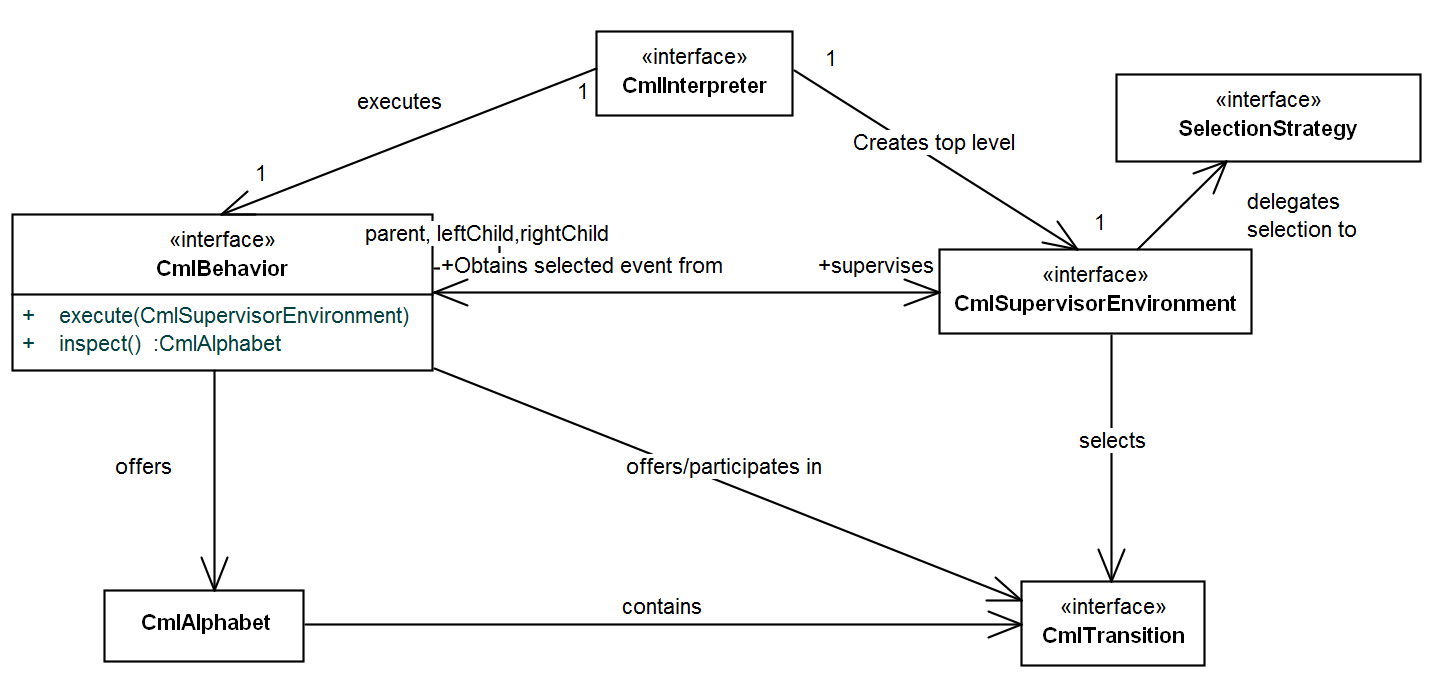
\includegraphics[width=0.9\textwidth]{figures/toplevelStructure}
    \caption{Diagram depicting the high level design of the interpreter core component}
    \label{fig:interpreter_topLevelStructure}
  \end{center}
\end{figure}

\begin{description}
\item[CmlInterpreter] The main interface exposed by
  the interpreter component. This interface has the overall
  responsibility for interpreting. It exposes methods to execute, listen
  on interpreter events and get the current state of the interpreter. It
  is implemented by the \textbf{VanillaCmlInterpreter} class.

\item[CmlBehaviour] Interface that represents a
  behaviour specified by either a process or action. It exposes two
  methods \emph{execute} which performs the behaviour and
  \emph{inspect} which returns the immediate alphabet of the
  behaviour. A specific behaviour can for instance be the Skip action,
  which when executed successfully terminates the action.
\item [CmlSupervisorEnvironment] Interface with the
  responsibility of acting as the environment for processes and
  actions. This involves choosing the next event (if any) given the
  available events. It has a method for retrieving the occurring
  event.
\item[CmlEvent] Interface that represents any kind of event. This
structure will be described in more detail in section
\ref{sec:event_structure}
\item[CmlAlphabet] This class is a set of CmlEvents.
\item[CmlEventSelectionStrategy] This interface has the responsibility
  of choosing one event from a CmlAlphabet
\end{description}

\subsubsection{Event Structure}
\label{sec:event_structure}

\subsection{Dynamic Structure}
\label{sec:dynamic_structure}


%%%% Bibliography %%%%
\newpage
\bibliographystyle{alpha}
\bibliography{bibliography} 
\label{ch:bib} %label to refer to


\end{document}  